% DATA 255 Final Project Report: IEEE Computer Society journal template (IEEEtran, compsoc).
% Build: pdflatex main && bibtex main && pdflatex main && pdflatex main
% Before submission: grep for \draft and remove every one; set \showdraftfalse.
\documentclass[10pt,journal,compsoc]{IEEEtran}

\usepackage[T1]{fontenc}          % clean text extraction for TurnItIn
\usepackage{graphicx}
\usepackage{booktabs}
\usepackage{tabularx}
\usepackage{array}
\usepackage{amsmath,amssymb}
\usepackage{url}
\usepackage{xcolor}
\ifCLASSOPTIONcompsoc
  \usepackage[nocompress]{cite}
\else
  \usepackage{cite}
\fi
\usepackage[hidelinks]{hyperref}

\graphicspath{{generated/figures/}{figures/}}

% Visible placeholders while drafting. Set \showdraftfalse for the final build.
\newif\ifshowdraft
\showdrafttrue
\newcommand{\draft}[1]{\ifshowdraft\textcolor{red}{[#1]}\fi}
% Pull a generated table or figure if it exists, otherwise show a placeholder.
\newcommand{\gen}[2]{\IfFileExists{generated/#1}{\input{generated/#1}}{\draft{#2}}}
% Same for a generated figure: \genfig{file.pdf}{caption}{label}{placeholder} (full text width, top of page).
\newcommand{\genfig}[4]{\begin{figure*}[t]\centering\IfFileExists{generated/figures/#1}{\includegraphics[width=\textwidth]{#1}}{\draft{#4}}\caption{#2}\label{#3}\end{figure*}}
\newcolumntype{Y}{>{\raggedright\arraybackslash}X}

\begin{document}

\title{Do Financial Vision Models Learn Price Patterns or Rendering Shortcuts? A Counterfactual Robustness Study of CNNs and Vision Transformers}

\author{Parth~Patel,~Khushi~Donda,~Farzaan~Dalwai,~and~Kaushik~Hariharan%
\IEEEcompsocitemizethanks{\IEEEcompsocthanksitem The authors are students in DATA 255, Deep Learning and Computer Vision, Fall 2026, San Jos\'e State University, San Jose, CA, USA.}}

\markboth{DATA 255 Final Project Report, Fall 2026}%
{Patel \MakeLowercase{\textit{et al.}}: Financial Vision Models and Rendering Shortcuts}

\IEEEtitleabstractindextext{%
\begin{abstract}
% Owner: Parth. Written last (Nov 23) from Tables 1 and 5. About 200 words.
\draft{Problem, method (counterfactual renderings, E1 to E5, augmentation and consistency controls), main measured results with metric and baseline, scoped conclusion.}
\end{abstract}

\begin{IEEEkeywords}
Financial chart images, shortcut learning, counterfactual rendering, robustness, vision transformers, convolutional neural networks, consistency regularization, calibration.
\end{IEEEkeywords}}

\maketitle
\IEEEdisplaynontitleabstractindextext
\IEEEpeerreviewmaketitle

% ---------------------------------------------------------------------------
\section{Introduction}\label{sec:intro}
% Owner: Parth | Draft Nov 21 | Final Nov 23 | 0.6 pages
\IEEEPARstart{C}{hart}-image models \draft{Motivation; the risk that models read rendering instead of prices; research questions RQ1 to RQ10; contributions list.}

% ---------------------------------------------------------------------------
\section{Related Work}\label{sec:related}
% Synthesize, do not list. IEEE numeric citations via \cite{}. At least 13 papers in total.
\subsection{Financial Chart-Image Prediction}   % Owner: Farzaan
\draft{3.1}
\subsection{Representation and Rendering Effects} % Owner: Farzaan
\draft{3.2}
\subsection{Shortcut Learning and Robustness}   % Owner: Khushi
\draft{3.3}
\subsection{CNN versus Transformer Robustness}  % Owner: Kaushik
\draft{3.4}
\subsection{Consistency and Invariance Training} % Owner: Khushi
\draft{3.5}
\subsection{Interpretability}                   % Owner: Kaushik
\draft{3.6}
\subsection{Calibration and Evaluation}         % Owner: Parth
\draft{3.7}
\subsection{Research Gap}                       % Owner: Parth
\draft{3.8: gap, then how our project addresses it.}

% ---------------------------------------------------------------------------
\section{Problem Formulation}\label{sec:problem}
% Owner: Parth | Draft Nov 20 | 0.3 pages
\draft{Window definition, label definition, the invariance question as a formal statement.}

\section{Dataset and Leakage Control}\label{sec:data}
% Owner: Farzaan | Draft Nov 21 | 0.7 pages | Sources: split_report.md, leakage test log
\draft{Universe, source, dates, splits, label thresholds, the 35-day purge and embargo derivation, test evidence that controls passed.}

\section{Counterfactual Rendering Method}\label{sec:render}
% Owner: Farzaan | Draft Nov 22 | 0.6 pages | Figure 1
\draft{R0 to R6, seen vs held-out, equivalence tests.}
\begin{figure*}[t]
\centering
\IfFileExists{generated/figures/fig1_renderings.pdf}{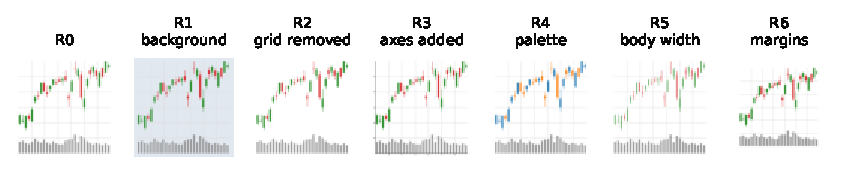
\includegraphics[width=\textwidth]{fig1_renderings.pdf}}{\draft{Figure 1: one window drawn in R0 to R6}}
\caption{One OHLCV window drawn in the seven renderings. Financial information is identical; only the named rendering factor changes.}
\label{fig:renderings}
\end{figure*}

\section{Models}\label{sec:models}
\subsection{ResNet-18 and the Shared Training Recipe} % Owner: Kaushik
\draft{7.1}
\subsection{DeiT-S and the Consistency Loss}        % Owner: Khushi
\draft{7.2}
\begin{equation}
\mathcal{L} = \tfrac{1}{2}\big[\mathrm{CE}(f(x_a), y) + \mathrm{CE}(f(x_b), y)\big] + \lambda\,\mathrm{JS}\big(p_a \,\|\, p_b\big)
\end{equation}

\section{Experimental Design and Ablations}\label{sec:design}
% Owner: Kaushik | Draft Nov 21 | 0.6 pages | Ablation matrix A1 to A8
\draft{Experiment matrix B0, E1 to E5; ablations A1 to A8; fairness controls for the CNN and ViT comparison; tuning budget and selection rules.}
\draft{Compute environment for reproducibility: a single NVIDIA GeForce RTX 5090 GPU for all image-model experiments (B0 and E5 on CPU), fp16 mixed precision, PyTorch and timm versions, seeds, epoch cap, optimizer, learning rate, batch size, checkpoint selection by validation Macro F1.}

\section{Evaluation Metrics}\label{sec:metrics}
% Owner: Parth | Draft Nov 21 | 0.6 pages
\draft{Predictive, robustness, reliability, stability, interpretability metrics; why each; the baselines each result is compared with.}

% ---------------------------------------------------------------------------
\section{Results}\label{sec:results}
% Numbers only from generated/ fragments. Every statement: metric, baseline, comparison, scope.
\subsection{Predictive Performance}             % Owner: Kaushik
\gen{tables/table1_main.tex}{Table 1: main results, generated}
\draft{10.1}
\subsection{Rendering Robustness and Interventions} % Owner: Khushi
\gen{tables/table2_per_render.tex}{Table 2: per-rendering sensitivity, generated}
\gen{tables/table5_comparisons.tex}{Table 5: planned comparisons A1 to A7, generated}
\genfig{fig3_flip_by_render.pdf}{Flip rate against R0 for each rendering factor (test split, mean $\pm$ SD over seeds). Shaded: held-out factors, never seen in training or tuning.}{fig:flip_by_render}{Figure 3: flip rate by rendering, generated}
\genfig{fig4_tradeoff.pdf}{Macro F1 on R0 against the held-out flip rate, one point per seed.}{fig:tradeoff}{Figure 4: F1 vs held-out flip rate, generated}
\draft{10.2}
\subsection{Calibration and Stability}          % Owner: Parth
\gen{tables/table4_seeds.tex}{Table 4: stability and cross-seed disagreement, generated}
\gen{tables/table7_calibration.tex}{Table 7: ECE and Brier, generated}
\draft{10.3}

\section{Interpretability and Error Analysis}\label{sec:interp}
% Owner: Farzaan | Table 3, Figures 6 and 7
\gen{tables/table3_masking.tex}{Table 3: masking by region, generated}
\gen{tables/table3b_link.tex}{Table 3b: attribution-to-flip AUROC, generated}
\genfig{fig6_attribution.pdf}{Attribution mass share divided by area share per region on R0 (Grad-CAM for ResNet-18, attention rollout for DeiT-S; seed-0 models, D15 sample). Dashed line: mass proportional to area.}{fig:attribution}{Figure 6: attribution mass ratio by region, generated}
\genfig{fig7_masking.pdf}{Mean $|\Delta p|$ when a region is filled with the background colour, against an area-matched random non-ink control (R0, seed-0 models, D15 sample).}{fig:masking}{Figure 7: masking vs area-matched control, generated}
\draft{11}

\section{Discussion}\label{sec:discussion}      % Owner: Khushi
\draft{12: interpretation using the predefined logic, scoped to tested renderings and setup.}

\section{Sustainability}\label{sec:sustain}     % Owner: Kaushik
\draft{13: SDG 9 (target 9.5) connection and its limits; measured compute footprint from the compute ledger.}
\gen{tables/table_ledger.tex}{Compute ledger, generated by scripts/compute\_ledger.py}

\section{Lessons Learned and Best Practices}\label{sec:lessons} % Owner: Farzaan
\draft{14: from docs/lessons\_learned.md.}

\section{Innovation and Publication Potential}\label{sec:innovation} % Owner: Khushi
\draft{15}

\section{Limitations}\label{sec:limits}         % Owner: Parth
\draft{16}

\section{Conclusion}\label{sec:conclusion}      % Owner: Parth
\draft{17}

\section*{CRediT Authorship Contribution Statement}
% Owner: Parth. Built from substantive technical ownership; confirm against git log and technical_owner fields at the results freeze.
\textbf{Farzaan Dalwai:} Conceptualization, Methodology, Software, Data curation, Validation, Investigation, Formal analysis, Visualization, Writing (original draft). Data curation, preprocessing, temporal splitting and leakage controls, counterfactual rendering pipeline, numeric baseline methodology, and masking analysis.
\textbf{Kaushik Hariharan:} Conceptualization, Methodology, Software, Validation, Investigation, Formal analysis, Visualization, Writing (original draft). Shared training infrastructure, ResNet-18 methodology and experiments, augmentation and consistency CNN experiments, and Grad-CAM analysis.
\textbf{Khushi Donda:} Conceptualization, Methodology, Software, Investigation, Validation, Formal analysis, Visualization, Writing (original draft). Vision Transformer methodology and experiments, consistency objective, $\lambda$-selection methodology, attention-rollout analysis, and robustness interpretation.
\textbf{Parth Patel:} Conceptualization, Methodology, Software, Validation, Formal analysis, Investigation, Visualization, Writing (original draft), Writing (review and editing), Project administration. Evaluation methodology, robustness metrics, calibration, statistical analysis, experiment integration, result synthesis, and report integration.
\draft{Refine to the work actually completed.}

% ---------------------------------------------------------------------------
\bibliographystyle{IEEEtran}
\bibliography{references}

% ---------------------------------------------------------------------------
\appendices

\section{Rubric Evidence}\label{app:rubric}
% Owner: Parth. Same order as the rubric. Every claim needs evidence the teaching team can open.
\begin{table*}[!t]
\centering
\caption{How each rubric criterion was met}
\label{tab:rubric}
\small
\begin{tabularx}{\textwidth}{@{}p{2.6cm}YYp{3.6cm}@{}}
\toprule
\textbf{Criterion} & \textbf{How we met it} & \textbf{Evidence} & \textbf{External link or file} \\
\midrule
1. Report (7) & \draft{IEEE template, page count, size, grammar review} & \draft{PDF page count and size} & \draft{Canvas submission} \\
2. Sustainability (5) & \draft{SDG 9 mapping; compute footprint} & Section~\ref{sec:sustain} & \draft{compute ledger link} \\
3. Lessons learned (5) & \draft{Shared log; Section 14} & Section~\ref{sec:lessons} & \draft{GitHub docs/lessons\_learned.md} \\
4. Publication or competition (3) & \draft{Novelty, needed experiments, venues} & Section~\ref{sec:innovation} & \\
5. Innovation (5) & \draft{Counterfactual renderings, held-out factors, controls} & Sections~\ref{sec:render}, \ref{sec:design} & \\
6. Evaluation of performance (5) & \draft{Metrics, baselines, ablations, seeds, masking} & Sections~\ref{sec:metrics} to \ref{sec:interp} & \draft{GitHub outputs/eval} \\
7. Technical difficulty (7) & \draft{Technical inventory} & Appendix~\ref{app:technical} & \draft{GitHub repository} \\
8. LaTeX (1) & Native IEEE LaTeX source & Source files submitted & \draft{Canvas source zip} \\
9. Literature survey (5) & \draft{Number of papers, subsections, gap} & Section~\ref{sec:related} & \\
\bottomrule
\end{tabularx}
\end{table*}

\section{Generative AI and Tool Use Disclosure}\label{app:genai}
% Owner: Khushi. Built from docs/ai_use_log.md. Only tools actually used.
\draft{One paragraph on what AI tools were and were not used for, then the table.}
\begin{table*}[!t]
\centering
\caption{AI and tool use}
\label{tab:genai}
\small
\begin{tabularx}{\textwidth}{@{}p{1.7cm}p{2.2cm}p{2.9cm}YYY@{}}
\toprule
\textbf{Date} & \textbf{Member} & \textbf{Tool and model} & \textbf{Purpose and prompt category} & \textbf{Artifact affected} & \textbf{Human verification} \\
\midrule
2026-11-19 & Parth Patel & Claude (claude.ai), Claude Opus 5.5 & Project planning from the team specification and rubric & Execution plan, starter documentation, this skeleton & \draft{reviewer and checks} \\
\bottomrule
\end{tabularx}
\end{table*}

\section{Technical Inventory and Supplementary Results}\label{app:technical}
% Owner: Kaushik (inventory, compute ledger); Parth (per-seed tables); Farzaan (split report, test summary)
\draft{Modules, tests passed, compute ledger, per-seed tables, deviations log.}

\end{document}
